\section{Introduction}

Capturing section of the screen might seems a simple tasks, but it is often hidden away behind lesser known shortcuts or small apps and not necessarily commonly known. We tried to use the voice to help with such task.

\section{Outline}

By bringing the voice to help us with the task, we're not trying to be necessarily faster than using the different options already there, but we're focusing on adding a vocal to different small tasks to complement the standard usage in a connected world.
Inspired by different solutions used to take screenshots, our concept is relatively straight forward: the user will speak a command to start the selection, drag their mouse over a portion of their screen and then speak a second command word to have it capture.

\subsection{CASE/CARE}
\begin{figure}[H]
    \centering
    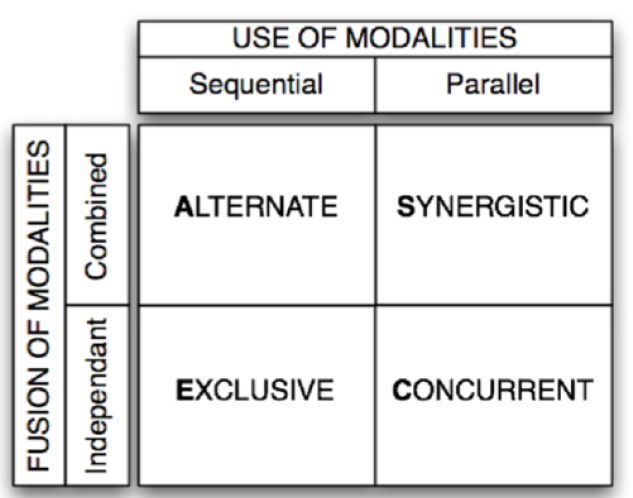
\includegraphics[scale=.6]{Report/images/CaseCare.png}
    \caption{CASE model}
    \label{fig:my_label}
\end{figure}

The utility will require them to use mouse, keyboard and voice in a \textbf{synergistic fashion} in the CASE model.
The position of the mouse is grabbed as the voice command is activated.

For the user, both applications are used \textbf{complimentary}.
As the mouse position will define the section selected when the words are spoken. 

\section{Architecture}
We went with Python for its strength in quick prototyping, good turnaround, extensive library and tools available across and our personal skills and knowledge.
Which turned out to be really helpful.

\subsection{Implementation}
\subsubsection*{Push to talk}
To limit as much as possible the social impact of our idea/software (to give instruction to the machine while being in an office), we chose to integrate a trigger functionality. The program can run as a background process on a machine and it is only triggered when a defined key (or combination of keys) is pressed. This way the users can speak as freely as they want, and when they need the screenshot functionality, they just have to enter the good shortcut to start the listening of their command and give their input  through a microphone to the computer.

\subsubsection*{Voice recognition}
The main part of the project is obviously the voice.
For this aspect, we used the speech recognition library with the Google Cloud Speech API.
The speech recognition function listens for some audio input from the user and then convert it to text. Once we have the text, we can seek for keywords to then execute the rest of the code.
In our case we decided to put this speech recognition function in a while loop. This way, once the program is started, it runs until the two commands are input and the screenshot is taken. This decision allows the user to make mistakes and retry.

For our keywords, we chose the words "from" and "there". Even though they are commonly used words, with our trigger functionality, we can limit the number of interferences from usual conversations.
Once the speech recognition finds those words it stores the position of the mouse pointer and once both positions (at "from here" and "to there") are known, they are sent to the screen capture function.

\subsubsection*{Screen capture}
Capturing the section of the screen turned out to be fast and direct. We simply saved the position of the mouse pointer at two moments (matching with the oral commands) and gave them to the screenshot function. Thanks to a library called PIL (more specifically a forked named Pillow) capturing a screenshot is a couple of lines of codes. 

\lstinputlisting[language=python, firstline = 150, lastline = 159, breaklines=true]{../voicegrab.py}

To use the screenshot, we took advantage of a library allowing us to directly save pictures to the Windows clipboard, which prevents us from using it cross platform. 

\subsubsection*{Comfort and feedback}
As we started to test our program from a text editor, we first went for textual feedbacks, with information about when the commands were not recognized, when the screenshot was successfully taken, etc.
But once we did our first user experience (requiring to take a screenshot on another window than the text editor) we quickly noticed that our first thoughts were not adapted to what we were looking for.

In order to stay in the voice world, and for utility purposes, we decided to pass these written feedbacks to audio ones. For this we used the Google Text to Speech library. This allowed us to have the computer say pre-registered sentences to the user while he was using our program.
We thus created audio clips for almost every cases in order to get the user notified of what was happening, if any errors occurred, or if the screenshot was successfully saved for example.
This improved a lot the comfort of the user. This way, he could know what was going on while been focus on a task on another window.


\section{User evaluations and data analysis}
Due to the peculiar times we are living, we had only four users for this test. This is why we chose to do the "within group" method, which is a very powerful method.
Our four users had to fill a small google form asking some questions to have information about them, what part of the population they represented, how they usually took screenshots, etc.
After this, we asked them to perform two tasks:
\begin{itemize}
\item To take a screenshot of an image (defined part of the screen) with the way they were used to use.
\item And to take a screenshot of the same image, with our solution.
\end{itemize}
For both assignments, we registered the time they took as well as the number of steps needed to have the to do them.
And finally a small set of questions to have a qualitative feedback from the users.

For this project evaluation, we have as dependant variables:
\begin{enumerate}
\item the time to realise a screenshot
\item the number of steps needed
\item the method used in the first task
\end{enumerate}

As independent variables, we have:
\begin{enumerate}
\item the voice commands 
\item the modalities used (voice, keyboard and mouse).
\item the method used in the second task
\end{enumerate}

Before this evaluation we made two hypothesis based on the project goals, since we tried to increase the productivity in an office context.
\begin{itemize}
\item The first one is that our method would not be quicker than others.
\item The second one is that the number of steps needed to do a task would be smaller using our tool than using other/preferred tools.
\end{itemize}
\subsection{results}
\subsubsection*{Population and habits}
From our users, we had one retired person, one person in the working life and two students. Only one of the student usually worked with a Mac while the three other users were familiar with windows, but they all known a technique to take a screenshot.

For the method they used, the majority used the PrintScreen key on the keyboard and then used another software (in those cases Paint) to crop the image and select only the required content. The student using windows on a daily basis used the screenshot software integrated in windows and a combination of shortcuts to go faster.

Unfortunately, (or fortunately depending on the point of view) the first user test allowed us to detect bugs, big issues concerning the feedback of the program as well as the lack of good instructions on how our code should be used at the beginning of . Thanks to this, we could improve our program and test it with the three other users. This is the reason why we had to stop the test during the second task, but we still kept the qualitative feedback of this user.
\subsubsection*{Results for the first task}
As said above the majority of the users (over the four) used the PrintScreen shortcut with the Paint software to resize the screenshot to the image that was asked.
Half of them rated the practicality of this method 4/5, one person rated it 3/5 and the last user rated it 2/5, meaning that the majority found their techniques useful.
And they all knew where to find their screenshot afterwards.

\subsubsection*{Results for the second task}
Using our tool, they were more divided concerning the practicality of this method. Two of them rated it 4/5 and 5/5, and the two others (including the user that encountered problems with the code)  rated id 1/5 and 2/5.
And here again, they all knew where to find their screenshot afterwards.

\subsubsection*{Quantitative analysis}
Timing our task, we obtained the results of table \ref{table:time}. As predicted our method is slower by a wide margin. On average the preferred method is faster by a wide margin, mostly due to the issues the first and 3rd user had.
\begin{table}[H]
    \centering
    \begin{tabular}{l|l|l|l|l}
    Prefered Methode & 39  & 3  & 35  & 30 \\ \hline
    Voicegrab        & X & 30 & 180 & 60
    \end{tabular}
    \caption{Time (in s) take to capture and paste the image}
    \label{table:time}
\end{table}

For the number of action taken (see table \ref{table:actions}), our method do edge out the preferred one.
\begin{table}[H]
    \centering
    \begin{tabular}{l|l|l|l|l}
    Prefered Methode & 8 & 4 & 8 & 8 \\ \hline
    Voicegrab        & X & 4 & 4 & 4
    \end{tabular}
    \caption{Number of actions}
    \label{table:actions}
\end{table}


\subsection{Qualitative feedbacks}
After those experiences, we asked them which method they preferred, if they encountered difficulties, and if they would reuse our method.

The majority of the users preferred the alternative to our tool using voice.
This decision is due to the problems encountered. Firstly, the ambiguity of the word "take" in "take a screenshot from here to there", where it can mean both "capture" and "move to another place". and the lack of hints nor useful feedbacks of the first evaluation.

But also, from the accent of people who aren't native English speakers, that is not recognised by the speech recognition function. And the misinterpretation of the vocal feedback of the program.

And at the end, half of the users would reuse our tool while the other half prefer to stay with their methods.

\section{Conclusion}

During this project we hit a few hiccup and limitations making our utility less effective. 
The voice recognition is slow, which makes the usage of it slightly awkward.
It is a clear point where our utility can be improved.
But while slow is quite powerful and opens a lot of opportunities. 
Also we hope that our tester have learned how to take screenshot more effectively.

\subsection{Improvement paths}
Outside of a better UX through a clear GUI and feedback, there's a few clear paths for our applications.


We could relatively see an option where the utility could capture distinct windows, or start recording of small portion of the screen, through different triggers.
An option we studied was to integrate our voice detection and triggers with an open source app called \href{https://getsharex.com/}{ShareX} which offers a lot of options for this task.
We moved away from it for simplicity as we wanted to test the process more than the results.

Another path would be to have the screenshot process triggered by a keyword instead of pressing a key.
We didn't study the option to use trigger words with constant listening, but it is something people are more and more used to with the rise of different smart assistant. 

